\section{Auswertung}
\label{sec:Auswertung}
\paragraph{Verwendete Pendel}
Im ersten Durchlauf des Versuchs werden die Pendel der Längen $l_{1,l} = (58.23 \pm 0.47) \si{\centi\meter}$ und $l_{1,r} = (58.43 \pm 0.47) \si{\centi\meter}$ verwendet. Diese weisen im Mittel die Schwingungsdauern $T_{1,l} = (1.478 \pm 0.02) \si{\second}$ und $T_{1,r} = (1.466 \pm 0.014) \si{\second}$ auf.
Anschließend werden die Pendel $ T_{2,l} = (1.777 \pm 0.007)\si{\second}$ und $T_{2,r} = (1.779 \pm 0.038)\si{\second}$ eingestellt. Da die aufgezeichnete Pendellänge offensichtlich fehlerhaft ist wird hierraus die vermutete Länge auf $l_{2,l} =78.44 \si{\centi \meter}$ und $l_{2,r} = 78.616 \si{\centi\meter}$ berrechnet.

\paragraph{Gleichphasige und gegenphasige Schwingung}

Bei der gleichphasigen Schwingung ergeben sich $5 \cdot T_{1,+} = (7.228 \pm 0.177) \si{\second}$, also $T_{1,+} = (1.445 \pm 0.0354) \si{\second}$, sowie $T_{2,+} = (1.746 \pm 0.024) \si{\second}$ ($5 \cdot T_{2,+} = (8.73 \pm 0.12)\si{\second}$).

Bei gegenphasiger Schwingung ergeben sich $5 \cdot T_{1,-} = (6.42 \pm 0.184) \si{\second}$, also $T_{1,-} = (1.284 \pm 0.0368) \si{\second}$, sowie $T_{2,-} = (1.559 \pm 0.03) \si{\second}$ ($5 \cdot T_{2,-} = (7.795 \pm 0.150)\si{\second}$).

Dies entspricht $\omega_{1,+} = 2\pi / T_{1,+} = (9.08 \pm 0.22) \si{\hertz}$, bzw $\omega_{1,-} = (8.07 \pm 0.23) \si{\hertz}$. Analog ergeben sich $\omega_{2,+} = (10.97 \pm 0.15) \si{Hertz}$ und $\omega_{2,-} = (9.80 \pm 0.19) \si{\Hertz}$.
Aus \eqref{eqn:ggs} ergeben sich dann
\begin{equation*}
  K_1 =\frac{l}{2} \left(\frac{2\pi}{T_{1,-}} \right)^2-\frac{g}{2}= (700 \pm 40)\si{\meter\per\second\squared}
\end{equation*}
und
\begin{equation*}
  K_2 =   .
\end{equation*}
$\kappa$ hingegen ergibt sich zu:
\begin{equation*}
  \kappa_1 = \frac{T_{1,+}^2 - T_{1,-}^2}{T_{1,+}^2 - T_{1,-}^2} = 0.12 \pm 0.04
\end{equation*}

\begin{figure}
  \centering
  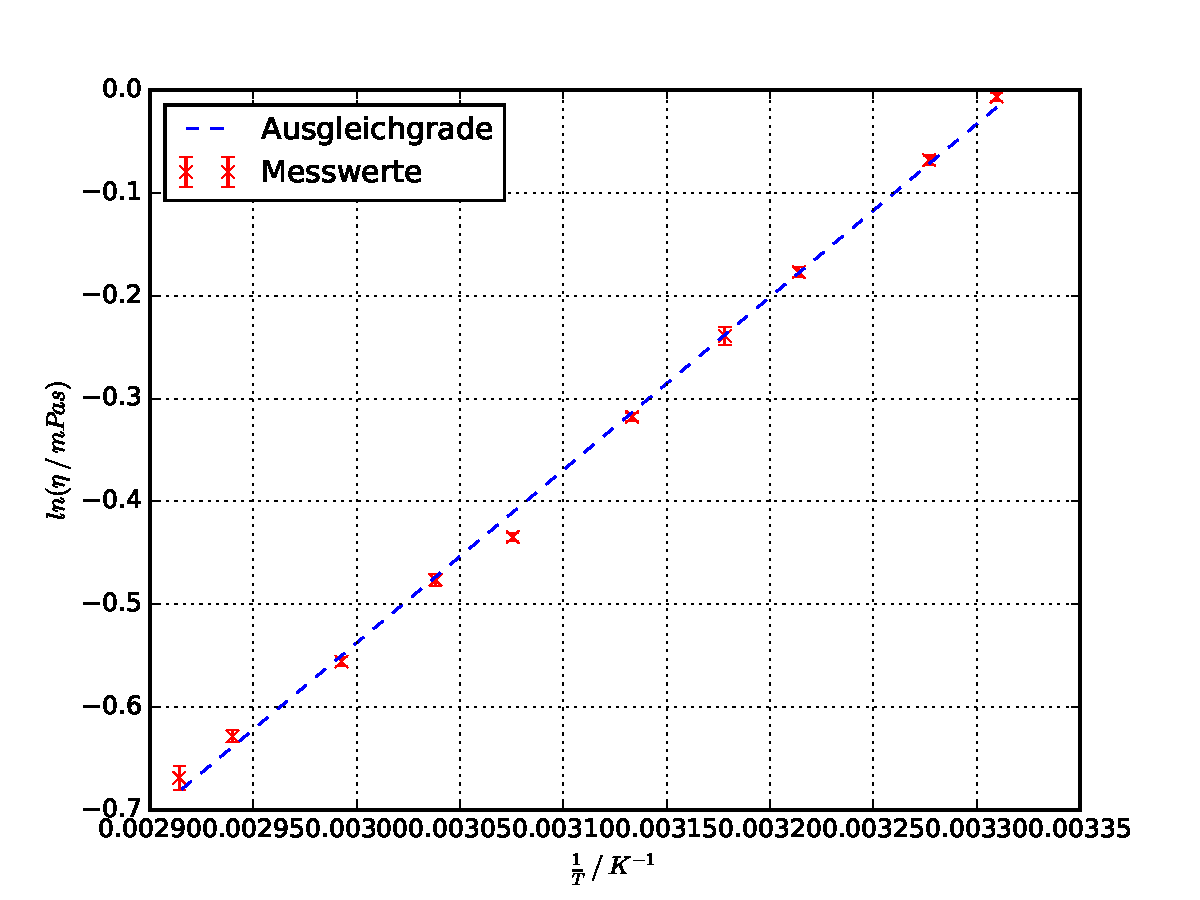
\includegraphics{plot.pdf}
  \caption{Plot.}
  \label{fig:plot}
\end{figure}
